%%%%%%%%%%%%%%%%%%%%%%%%%%%%%%%%%%%%%%%%%
% Simple Sectioned Essay Template
% LaTeX Template
%
% This template has been downloaded from:
% http://www.latextemplates.com
%
% Note:
% The \lipsum[#] commands throughout this template generate dummy text
% to fill the template out. These commands should all be removed when 
% writing essay content.
%
%%%%%%%%%%%%%%%%%%%%%%%%%%%%%%%%%%%%%%%%%

%----------------------------------------------------------------------------------------
%	PACKAGES AND OTHER DOCUMENT CONFIGURATIONS
%----------------------------------------------------------------------------------------

\documentclass[12pt]{article} % Default font size is 12pt, it can be changed here

\usepackage{geometry} % Required to change the page size to A4

\usepackage[utf8]{inputenc} % Use this package to enable the use of special norwegian characters (æ, æ, å)

\geometry{a4paper} % Set the page size to be A4 as opposed to the default US Letter

\usepackage{graphicx} % Required for including pictures

\usepackage{float} % Allows putting an [H] in \begin{figure} to specify the exact location of the figure
\usepackage{wrapfig} % Allows in-line images such as the example fish picture

\usepackage{cite}

\usepackage{url}

\usepackage{pdfpages}

\usepackage{supertabular} % Used for tables

\usepackage{tocbibind}

\usepackage[parfill]{parskip} % Newline without indent

\usepackage{lipsum} % Used for inserting dummy 'Lorem ipsum' text into the template

\usepackage{array}
\linespread{1.2} % Line spacing

%\setlength\parindent{0pt} % Uncomment to remove all indentation from paragraphs

\graphicspath{{./Pictures/}{./Pictures/Recordings/}} % Specifies the directory where pictures are stored

\setcounter{tocdepth}{5} %to make it appears in TOC
%\setcounter{secnumdepth}{5} %to make it numbered


\begin{document}
%----------------------------------------------------------------------------------------
%	TITLE PAGE
%----------------------------------------------------------------------------------------

\begin{titlepage}

\newcommand{\HRule}{\rule{\linewidth}{0.5mm}} % Defines a new command for the horizontal lines, change thickness here

\center % Center everything on the page

\textsc{\LARGE Høgskolen i Gjøvik}\\[0.5cm] % Name of your university/college
\includegraphics[width=90px, height=90px]{Logo}\\[0.8cm] % Include a department/university logo - this will require the graphicx package 403x403px
\textsc{\Large Data Communication And Network Security}\\[0.5cm] % Major heading such as course name
\textsc{\large Group Project}\\[0.5cm] % Minor heading such as course title

\HRule \\[0.4cm]
{ \huge \bfseries SSL - Secure Sockets Layer}\\[0.4cm] % Title of your document
\HRule \\[1.5cm]

\begin{minipage}{0.44\textwidth}
\begin{flushleft} \large
%\emph{Authors:}\\
Victor \textsc{Rudolfsson} - 120912\\ % Your name
Tommy \textsc{B. Ingdal} - 120913\\ % Your name
Dag \textsc{Jahren} - 120923\\ % Your name
Halvor \textsc{Thoresen} - 120915\\ % Your name
\end{flushleft}
\end{minipage}

\vfill % Fill rest of the page with empty lines
{\large \today}\\[3cm] % Date, change the \today to a set date if you want to be precise

\end{titlepage}

%----------------------------------------------------------------------------------------
%	TABLE OF CONTENTS
%----------------------------------------------------------------------------------------
\tableofcontents % Include a table of contents
\newpage % Begins the essay on a new page instead of on the same page as the table of contents 

%----------------------------------------------------------------------------------------
%	INTRODUCTION
%----------------------------------------------------------------------------------------
\section{Introduction} % Major section

\subsection{History} % Sub-section

In 1994 Netscape company developed the SSL protocol. This was made with the intention to make secure transmissions with an encrypted data path between a server and a client. To begin with, SSL was created mainly for web browsers and communications with servers.\cite{sslHist} \\
Netscape continued working on the SSL technology, and in 1995 they released SSL version 2.0. The problem with this version was that it had a lot of vulnerabilities which could have been exploited. Some of the weaknesses were even released in an article\cite{sslv2}. For example, one of the released vulnerabilities meant that if your host had already been compromised, SSL wouldn't do much to protect you. After a not-so-successful release of SSL 2.0, they reworked the protocol and tried to solve previous vulnerabilities. \\
In 1996 Netscape released SSL version 3.0. SSL 2.0 had a vulnerability which enabled outsiders to change/modify data during transmission, but this was fixed in SSL 3.0. Version 2.0 had MACs which was encrypted at 40-bit, while the new v3.0 keys were encrypted at 128 bits. Because of the improved security they implemented for authentication keys, SSL 3.0 was much more secure against i.e. hacking attempts. \cite{eHowSSL,sslHist}

\subsection{Introduction} % Sub-section

SSL is a protocol containing "rules" used for communication between a client and server. SSL uses authenticated and encrypted communication to establish a secure connection. The protocol runs as a layer between the Transmission Control Protocol and Application layer. The main "job" for SSL is to provide encrypt data being transmitted and decrypt data being received, which only the applications using it should be able to do.\cite{oracleIntro} It also provides detection of whether or not data has been changed/modified during transmission. Both parties agree on which algorithms to use for exchanging keys, authenticating one another, encrypting/decrypting the data, as well as checking its integrity; to make sure that detection of a third party changing/modifying the data will be possible.
Because of the encryption SSL provides by the use of strong algorithms, it allows for secure data communication, denying a potential third party to access the transmitted data.\cite{ibmIntro}
SSL uses authentication to make sure you know who you are communicating with, by the use of certificates and public key encryption, as well as allowing messages to be signed.\cite{oracleIntro}
For an SSL connection to be established, it's required to go through the “handshake”, in which the key exchange occurs. During this procedure, a pre-secret key is created and then subsequently turned into a master key to allow for symmetric encryption of the information transmitted through the SSL connection.\cite{how2ssl}
In this report, we'll try to explain these procedures, and we'll go over some of the algorithms used in both the handshake, as well as the encryption that follows. % Includes the file that contains the introduction

%----------------------------------------------------------------------------------------
%	SHORT DESCRIPTION OF PROTOCOL
%----------------------------------------------------------------------------------------
\section{Short Description Of The Protocol} % Major section

\subsection{SSL Handshake}
\begin{wrapfigure}{R}{0.4\textwidth}
	\vspace{-30pt}
  \begin{center}
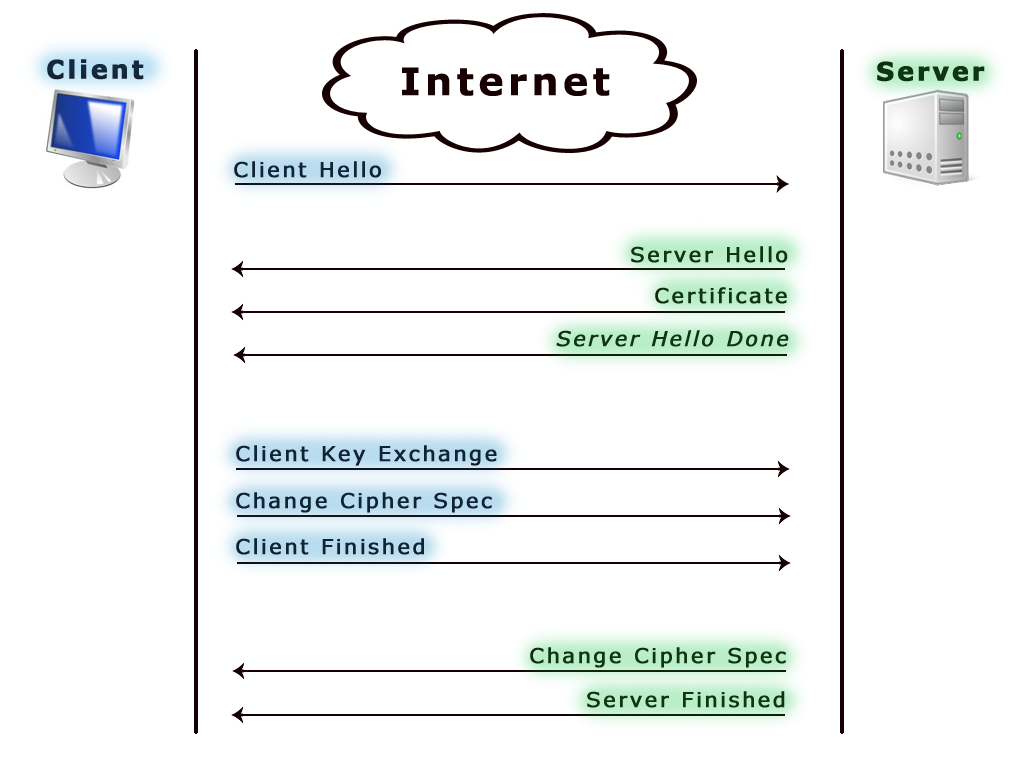
\includegraphics[width=0.50\textwidth]{SSL_handshake_image}
  \end{center}
	\vspace{-20pt}
  \caption{SSL Handshake}
\end{wrapfigure}
When you visit a website using the https protocol~\cite{wikipediaHTTPS} \textit{(technically not a protocol, since SSL/TLS is just layered on top of the HTTP protocol)}, the client and the webserver tries to establish a secure connection using SSL/TLS~\cite{wikipediaSSLTLS}. But before the secure connection is established, we have to perform a SSL handshake.\\ 
However, in order to complete a SSL handshake, the client and the server has to complete a number of steps, some of which are optional. And if for some reason a problem occurs in the negotiation, the connection is usually dropped.\\\\
In this section we will give a brief overview of how the SSL handshake is completed and how it makes your communication with the web server secure.

\subsubsection{9 Steps To Secure Communication}
\begin{enumerate}
\item The client sends a ClientHello message to the server. This message contains information about which version the client supports, some randomly generated data and a list of all the cipher suites the client supports.
\item The server will now respond with a Server Hello message which include the highest version number both sides support, some randomly generated data and the cipher suite chosen by the server. It is worth mentioning that the cipher suite chosen by the server is the strongest suite both sides supports.
\item Now the server will send its certificate to the client. The server's public key is stored inside this certificate, and is used by the client to authenticate and encrypt the premaster key.
\item At this point the server is done, and waits for a response from the client.
\item It is now time to start exchanging keys. In step 1 and 2 both the client and the server sent some random values to each other. These random values is now used to generate the premaster secret. After the premaster secret is generated, it is encrypted using the server's public key and sent back to the server.
\item The client now sends a Change Cipher Spec message to the server, which basically says that all data being sent from the client from now on will be encrypted.
\item To finish the negotiation from the client's side, a Client Finished message is sent to the server.
\item The server now respond with a Change Cipher Spec message and tell the client that all data sent from the server from now on will be encrypted.
\item To complete the negotiation the server sends a Server Finished message back to client. And if everything went well the SSL handshake is now finished and a secure channel is initiated between the client and the server.
\end{enumerate}
This is obviously a very brief overview of how the SSL handshake works. But in section 4, Bit-Level Description, we will go into more detail about the handshake, and also explain exactly what kind of data and values are being transmitted from the client to the server, and vice versa.

%----------------------------------------------------------------------------------------
%       GLOBAL DESCRIPTION
%----------------------------------------------------------------------------------------
\section{An Overview Of SSL}
\subsection{Global Description}
\begin{wrapfigure}{R}{0.5\textwidth}
	\vspace{-30pt}
  \begin{center}
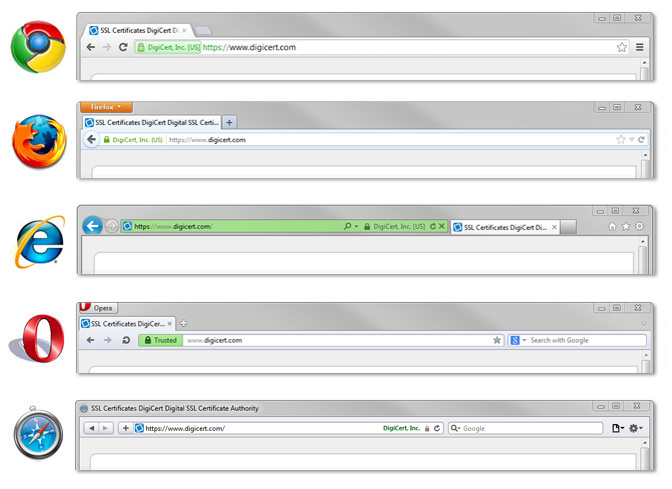
\includegraphics[width=0.60\textwidth]{browservisualq}
  \end{center}
	\vspace{-15pt}
  \caption{Visual cues\cite{browservisualcues}}
\end{wrapfigure}

\subsubsection{Advantages}
The use of internet has drastically increased over the years and so has the different uses of the internet. This has demanded a huge increase in internet security.
As a result of this the use of SSL and TLS has become very popular and quite normal. Even though these security protocols are used all over the internet, it's still a topic almost nobody got any knowledge of. So how does SSL help a website if the users don't know how it works, or what it does? Well, the whole SSL certificate system is built around trust. The only thing the users/customers have to know, is that if a website is secures with SSL, it means that it is safe to use that website. Since the most important part for a website is to show the users that it is in fact safe to use, the universal symbol of safety, a lock, or the color green is added to the address bar of any website that has a valid SSL certificate, as seen in figure 3. 
This ensures the users that a certificate authority, or CA for short,  has reviewed the website and made it safe to use and can be trusted. \cite{digicert}\\
But why is it so important for a company's and websites to have the users trust them? 
The media has for the last couple of years focused a lot on internet security. Because of this more and more people are aware of the risk they take when sending information over the internet. And if they can ensure their users that it is in fact safe, then it is more likely that the user will use the services on their website.\\
Another important advantage for a company to have a SSL certificate is that it reduces the amount of successful phishing sites. This is because it is very difficult for criminals to get a valid SSL certificate on their phishing site.\cite{sslshopper}\\

\subsubsection{Disadvantages}
Even though there are a lot of advantages with using SSL, there are also a couple of disadvantages that companies have to consider before getting a SSL certificate. One of the biggest disadvantages is the fact that getting a SSL certificate can be quite costly. This is because SSL providers have to ensure that their customer's website is secured and validate their identity. And since most companies buy SSL certificates to get more customers and earn more money, it might not be worth getting because of the implementation cost. \cite{sslshopper}\\
Another disadvantage is the fact that encrypting the information takes more resources, and decreases the server performance. Even though this decrease in performance is minimal, it might cause trouble for sites with a lot of traffic. There is also special hardware that can minimize the performance decrease, but that might again not be very cost efficient for the company.  \cite{sslshopper}


%----------------------------------------------------------------------------------------
%       CERTIFICATE AUTHORITY
%----------------------------------------------------------------------------------------
\subsection{Certificate Authority}
\subsubsection{Introduction}
When we talk about a Certificate Authority we talk about a trusted third party that issues Digital Certificates. These certificates are used to digitally sign messages that identifies the sender.\\
We can compare this digital signature with a written signature. The purpose is to guarantee that the sender actually is who it claims to be.\\
But since signatures can be forged, digital signatures offers a number of different encryption algorithms to minimize this risk and offer the client and server a safe way to communicate across the Internet.
\subsubsection{Issuing A Certificate}
Certificate Authorities offers a few ways to verify the validity of an entity when they request a certificate. One way is to do a domain validation - this is the least secure way of verifying that the entity actually is who it claims to be.\\
The second method is to do an extensive validation of the entity, thus ensuring the users that the website really can be trusted.
\subparagraph{Domain Validation}~\\
Like it says above this section, domain validation is the least secure way of validating an entity.\\
This is because the CA (Certicate Authority) only uses the domain to verify an entity. Whatever information they find doing a WHOIS is included in the certificate, and thus trusted by the CA.\\
This means that even though the certificate still uses 128-bit encryption, phishers can obtain a certificate and hide their identity.\\
And if you combine this with a MITM (man-in-the-middle) attack, an attacker can use DNS poisoning and use a domain validated certificate for your domain and redirect users to a fake site, thus enabling the attacker to obtain and collect sensitive user information.
\subparagraph{Extensive Validation}~\\
With an Extensive Validated Certificate you get alot more security for your users. EV Certificates are designed to prevent phishing attacks better than normal domain validated certificates.\\
The extensive validation~\cite{EVCert} checks quite a few different aspects of your organization, including:
\begin{itemize}
	\item Verifying that the organization is registered and active
	\item Verifying that the organization has exclusive rights to use the domain
	\item Verifying that the organization is not on any government blacklists
\end{itemize}
Even though this certificate is more expensive than the normal certificate, it is obvious that it provides many more benefits and that this certificate is the right choice if you really want to ensure the safety for your users.
\begin{wrapfigure}{R}{0.35\textwidth}
	\vspace{-30pt}
  \begin{center}
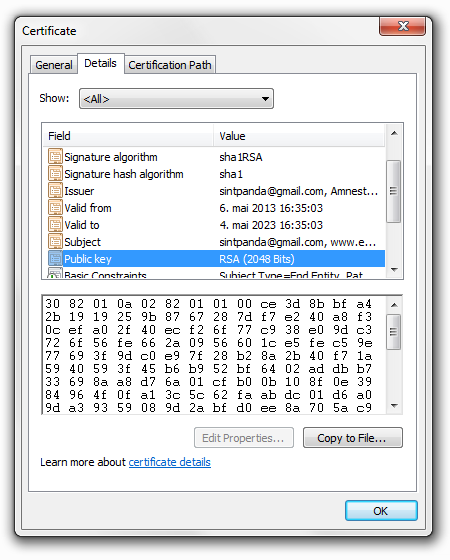
\includegraphics[width=0.40\textwidth]{endusercert}
  \end{center}
	\vspace{-20pt}
  \caption{Client Certificate}
\end{wrapfigure}
\subsubsection{Certificate Structure}

In this section we will briefly go through the structure of an end user certificate and a root certificate.\\
Even though the two certificates does have some fields which are the same, there are a few key differences between them.
\subparagraph{End user certificate}~\\
The end user certificate or, client certificate, basically is the certificate which gets installed on the client's computer.\\
\\
\emph{Version}
\begin{itemize}
	\item This field contains information about the certificate's version. Today there are three versions; 1, 2 \& 3. Higher certificate versions can contain more fields and information.
\end{itemize}
\emph{Serial number}
\begin{itemize}
	\item When the CA issues a certificate, they assign a unique integer to the certificate. This ID has to be unique for each certificate.
\end{itemize}
\emph{Signature algorithm}
\begin{itemize}
	\item Client and servers can communicate using a large range of different encryption algorithms. This field contains the algorithm identifier used by the CA to sign the content using the private key.
\end{itemize}
\emph{Signature hash algorithm}
\begin{itemize}
	\item This field contains information about which hash algorithm to use to hash the content before signing.
\end{itemize}
\emph{Issuer}
\begin{itemize}
	\item In this field we can see information about the entitiy that issued the certificate. For instance; ''C = NO'' means that the issuer is located in Norway (NO) and ''O = Dundergruppen'' is the name of the organization. 
\end{itemize}
\emph{Valid from}
\begin{itemize}
	\item Information about the date the certificate is valid from.
\end{itemize}
\emph{Valid to}
\begin{itemize}
	\item Information about the date the certifiicate is valid to.
\end{itemize}
\emph{Subject}
\begin{itemize}
	\item This field contanins information about the CA that created, issued and signed the certificate.
\end{itemize}
\emph{Public key}
\begin{itemize}
	\item Here we can see the public key and information about the algorithm used.\\
Example:\\
RSA (2048 Bits)\\
''\textit{30 82 01 0a 02 82 01 01 00 ce 3d 8b bf a4 2b 19 19 25 9b 87 67 28 7d f7 e2 40 a8 f3 0c ef a0 2f 40 ec f2 6f 77 c9 38 e0 9d c3 72 6f 56 fe 66 2a 09 56 60 1c e5 fe c5 9e 77 69 3f 9d c0 e9 7f 28 b2 8a 2b 40 f7 1a 59 40 59 3f 45 b6 b9 52 bf 64 02 ad db b7 33 69 8a a8 d7 6a 01 cf b0 0b 10 8f 0e 39 84 96 4f 0f a1 3c 5c 62 fa ab dc 01 d6 a0 9d a3 93 59 08 9d 2a bf d0 ee 8a 70 5a c9 3f 1f 15 b3 36 eb 67 15 e1 8e 5a c5 09 a7 84 bf 31 da a9 07 bf d4 e9 cd 2e 3f a5 e6 03 01 01 d6 67 b2 2b 92 84 06 84 f5 5f e0 d1 d7 5d e8 b0 e9 13 c5 07 db a3 86 5b 73 2f 07 f3 10 aa a4 79 ad e1 00 eb 8d 28 ce 3f ad f5 da 20 a6 f2 36 ef 88 b6 a7 93 9a f4 12 41 ca 99 96 5e 87 31 dd b5 78 d1 2d 83 bd 18 bc ac b2 f9 38 54 68 a3 b9 bb 3d ab 0a a3 6c e1 5c e7 7a d8 10 53 db bb 4d 1c 3d 2e 95 a2 0f 62 d6 ec 53 6f 38 25 02 03 01 00 01}''
\end{itemize}
\emph{Basic Constraints}
\begin{itemize}
	\item If the certificate can be used as a CA it is specified in this field. If not it is specified that the certificate is an ''End Entitiy''.
\end{itemize}
\emph{Key Usage}
\begin{itemize}
	\item Contains information about which operations the public key can be used for.\\
For instance: Digital Signature.
\end{itemize}
\emph{Thumbprint algorithm}
\begin{itemize}
	\item Specifies the algorithm used to hash the certificate.
\\For instance: SHA-1.
\end{itemize}
\emph{Thumbprint}
\begin{itemize}
	\item This is the hash itself. Basically used as an identifier.
\end{itemize}
\subparagraph{Root Certificate}~\\
\begin{wrapfigure}{h}{0.35\textwidth}
	\vspace{-30pt}
  \begin{center}
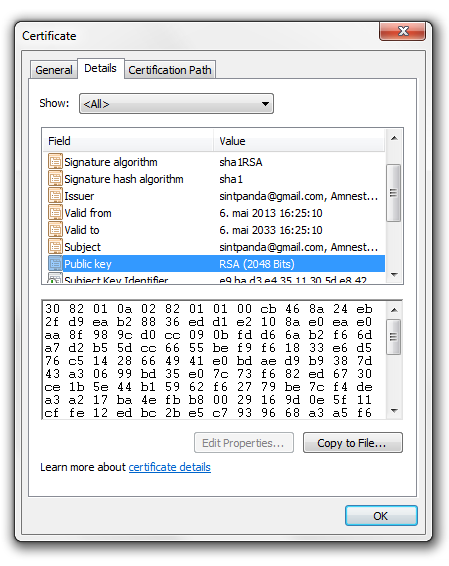
\includegraphics[width=0.40\textwidth]{rootcert}
  \end{center}
	\vspace{-20pt}
  \caption{Root Certificate}
\end{wrapfigure}
Like we mentioned earlier, end user certificates and root certificates contains many of the same fields and values.\\
It is however worth mentioning that the public key is exactly the same in both certificates. This because the client and server use a PKI (Public-key infrastructure)-modell.\\
However, there are differences, and in this section we will go through the field and values that differ between the two certificates.\\\\
\emph{Serial number}
\begin{itemize}
	\item This field contains a unique ID for this root certificate. This is used to distinguish between multiple certificates.
\end{itemize}
\emph{Subject Key Identifier}
\begin{itemize}
	\item This field contains an ID which provides a method of identifying certificates that contain a specific public key. A 160-bit SHA-1 hash of the value of the subjectPublicKey.
\end{itemize}
\emph{Authority Key Identifier}
\begin{itemize}
	\item To help verify the signature on this certificate, this field contains the public key used for that purpose.
\end{itemize}
\emph{Basic Constraints}
\begin{itemize}
	\item Since this is a Root Certificate this field contains the value ''Subject Type=CA''.
\end{itemize}
\subsubsection{Providers}
Worldwide there are a number of certificate authories, and the business is fragmented with national and regional providers.\\
However, certificates used for website security is largely held and issued by a small number of companies, and as of today more than 50 root certificates are trusted in the most popular web browers.\\\\
The market share between the top CA's, from W3Techs survey 2012, shows the following:
\begin{itemize}
	\item{Symantec (including VeriSign, Thawte \& GeoTrust) with 42.9\%}
	\item{Comodo with 26\%}
	\item{GoDaddy with 14\%}
	\item{GlobalSign with 7.7\%}
\end{itemize}

\subsubsection{CA Compromise}
A certificate authority compromise (CA Compromise) is an incident where an attacker is able to use the private key of a CA to issue fake certificates.\\
The worst case scenario is when a Root Certificate Authority is compromised. If that happen the Root Certificate Authority must notify all the relaying parties who trust their certificate, so that the relaying parties can stop trusting that specific certificate.\\\\
If however an Intermediate Root Certificate Authority is compromised, the Root Certificate Authority must revoke those certificates. And obviously the entitiy that got compromised must replace those certificates immediately, since those certificates no longer can be used due to the revocation.

\subparagraph{DigiNotar Incident}~\\
On august 30, 2011, DigiNotar confirmed~\cite{diginotarIncident} that they had been compromised and that Google.com certificates was obtained by the attackers.\\

``\emph{What at first appeared to be a one-off attack targeting Google Gmail users was actually part of a larger breach at Dutch digital certificate authority (CA) DigiNotar, which today confirmed speculation that it indeed was hacked and its SSL and EV-SSL CA system abused by attackers.\\
"The company found out on July 19 that a hacking attempt had happened. At that moment, DigiNotar ordered an external security audit. This audit concluded that all fraudulently issued certificates were revoked. We found out yesterday, through Govcert, that the Google certificate was active. We revoked it immediately," said a spokesman today at Vasco Data Security International, of which the Dutch DigiNotar is a wholly owned subsidiary.}''
% Source: http://www.darkreading.com/attacks-breaches/digital-certificate-authority-hacked-doz/231600498

\subparagraph{Consequences Of A Compromise}~\\ % Følger av en compromise
The CA paradigm is basically a chain-of-trust. So what happens when a CA experience a compromise?\\
If an attacker obtains a certificate for ex. Gmail.com, the attacker can basically impersonate Gmail by issuing forged certificates to its users with the purpose of stealing sensitive information and/or credentials - the trust is then broken.
\\\\
Most operative systems include a feature that will automatically update the system when the developers issues a patch or an update. The common thing is to use certificates to ensure the integrity of the patch, so no malware get's installed on the users system.\\
What happens if an attacker can inpersonate Microsoft and digitally sign his own files using Microsoft's credentials? Well, if an attacker combines that with DNS Poisoning your operative system will see the file issued by the attacker as a legitimate file and install it, thus potensially installing malware on your system.\\
This can obviously be used to steal sensitive information, credentials and/or use the compromised computer in a botnet.

%----------------------------------------------------------------------------------------
%	BIT-LEVEL DESCRIPTION
%----------------------------------------------------------------------------------------
\section{A Deeper Understanding} % Major section

Since encryption of data is one of the responsibilities of the transport
layer, it's important to mention that this is where encryption such as SSL/TLS (if used) operates. This has a very useful effect which benefits the protocol greatly: Because the transport layer is responsible for establishing connections as well, a connection will simply not be established if the security checks aren't passed.

The SSL / TLS procedure consists of two steps; the first one being authentication, and the second being encryption. Because SSL/TLS is based on the use of certificates, certificates is a very vital part of the process. One key difference (pun intended) between SSL and TLS, is that SSL requires the \textbf{server }to prove its identity to the client, whereas TLS requires both parties to prove their identity. 

\subsection[Handshake]{Handshake}
The first thing that needs to be done to initiate encryption is what we
call the 'handshake'. This is the first of the two processes that make up the SSL/TLS protocols, and in turn consists of several steps. 

The first step in the handshake process is called the negotiation phase.
During this phase, each packet contains a specific \textit{message type code}, which indicates what type of packet is being sent. 

First, the client sends a 'hello' to the server, this is called the \textit{ClientHello} (message type 1).
Listed within this 'hello' message is the algorithms (\textit{Cipher Suites}) which the client supports for encryption, allowing the server to pick the strongest supported algorithm and reply with the server's equivalent to ClientHello, namely \textit{ServerHello }(message type 2), containing a random number, the protocol the server has selected from the list of suggestions from the client, a random number, the CipherSuite, and compression method selected; followed by the server's x.509 certificate (message type 11) containing its public key. It's important to note that the server should always select the strongest available protocol.

When the negotiation is complete, the server will send a message indicating that it is done, called the \textit{ServerHelloDone} (message type 14) packet, to which the client will respond with a packet called the \textit{ClientKeyExchange}\cite{rfcClientKeyExchange,rfcSSLClientKeyExchange} (message type 16). This packet contains either a \textit{PreMasterSecret }\cite{rfcSSLPreMasterSecret} (encrypted with the public key found in the server's certificate), a public key, or nothing at all depending on the selected protocol\cite{rfcCipherSuiteDefinition,rfcCipherSuiteList}.

The random numbers contained within the \textit{ClientHello}\cite{rfcClientHello,rfcSSLClientHello} and \textit{ServerHello}\cite{rfcServerHello,rfcSSLServerHello} will be used to calculate a \textit{MasterSecret} together with the \textit{PreMasterSecret }in the next step. The \textit{MasterSecret} becomes a shared secret between the client and the server, which the data required for encryption will be based on.

When this is complete, both parties are ready to start encrypting data. This begins after the client sends a \textit{ChangeCipherSpec}\cite{rfcChangeCipherSpecProtocol,rfcSSLChangeCipherSpecProtocol} packet, essentially indicating that \textit{{\textquotedblleft}Now this side is ready to change to the cipher suite we have agreed to use, with parameters we calculated{\textquotedblright}, }and finally a \textit{Finished}\cite{rfcFinished,rfcSSLFinished} message containing the \textit{message authentication code}\cite{rfcSSLMAC} and hash calculated from the previous handshake messages.

Upon receiving this from the client, the server in turn responds with a similar \textit{ChangeCipherSpec} message indicating that it, too, is ready to start encryption of data, followed by a \textit{Finished} (message type 20) message.

Let's have a closer look at each of these messages:

\begin{description}
	\item[ClientHello]\cite{rfcClientHello,rfcSSLClientHello} This packet is required to be sent by the client as soon as it connects to the server, but can also be sent as a response to a ClientHelloRequest packet (such a packet is sent by the server if it wants to initiate renegotiation of the session - it's the server's way of saying "Hey, can we renegotiate? You start!" - but it's the client's responsibility to start the process with a ClientHello message). This packet should contain the following values/parameters:
	\begin{itemize}
		\item cipher\_suites: This parameter consists of the list of \textit{cipher suites} supported by the client, ordered by the client's preference (first to last). If none of the cipher suites suggested by the client is supported by the server, a handshake failure alert will be returned and the connection will be closed. We'll elaborate further on what a cipher suite actually in following sections.
		\item client\_version: This parameter indicates which the most recent version of the SSL/TLS protocol the client supports is (actually the version the client wishes to use, but these should be synonymous, as the client is required to suggest using the most recent version it supports).
		\item compression\_methods: This parameter contains a list of compression methods supported by the client, ordered first-to-last by the client's preference.
		\item extensions: This parameter is optional, and may be sent if the client wishes to request extended functionality. Servers are required to accept ClientHello packets both \textit{with} and \textit{without} this field supplied, but it's up to the client to decide whether or not it wants to abort the connection if the server does not support the requested extended functionality. Each extension suggested by the client should contain two fields, these being:
		\begin{itemize}
			\item extension\_type: The type of the extension being suggested
			\item extension\_data: Specific information regarding the specified extension type.
		\end{itemize}
		\item gmt\_unix\_time: This value contains the current UTC time stamp of the client's internal clock.
		\item random\_bytes: This value should be 28 randomly generated bytes by a secure random number generator. This value together with the random\_bytes value makes up the \textit{random parameter}.
		\item session\_id: This value holds the session ID, or nothing if it's either 1) not yet defined by the server (i.e. a handshake has not been completed) or 2) the client wants to renegotiate its security parameters.
	\end{itemize}
	
	\item[ServerHello]\cite{rfcServerHello,rfcSSLServerHello} This packet is sent as a response to the ClientHello message, after the server has chosen which algorithms it wishes to use from the suggestions made by the client in the preceding ClientHello message. This packet, not unlike the ClientHello, carries some data with it - although rather than suggesting several alternative algorithms, it confirms which ones will be used. Let's have a closer look at these fields:
	\begin{itemize}
		\item cipher\_suite: This field should contain the cipher suite selected by the server from the list supplied by the client in the preceding ClientHello message.
		\item compression\_method: Similarly, this field should contain the compression method selected by the server from the list of suggestions sent with the ClientHello message.
		
		\item extensions: This field should contain a list of extensions supported by the server - if (and only if) they were suggested by the client in the ClientHello message. It should serve as a response to the client's way of saying "I request the following additional features: ", by saying "... and of those you requested, I support these: ".
		
		\item gmt\_unix\_time: The current UTC time stamp of the server's internal clock.
		\item random\_bytes: 24 bytes randomly generated by a secure random number generator. Just like in the ClientHello message, this value together with the gmt\_unix\_time value makes up the \textit{random} parameter.
		
		\item server\_version: This field contains that suggested by the client in the preceding ClientHello message, and the highest version of the SSL/TLS protocol supported by the server.
		 
		\item session\_id: This field contains the unique ID for this session. If one that exists in the server's session cache was suggested by the client in the preceding ClientHello message and the server is willing to resume that session, it will respond with the same session ID. However, if that is not the case a new value will be created - unless the session cannot be resumed, in which case this field will remain empty. 
	\end{itemize}
	
	\item[ServerHelloDone]\cite{rfcServerHelloDone,rfcSSLServerHelloDone} This message is sent by the server when it's done sending the ServerHello and messages associated with it. It indicates that no more messages will be sent to support the key exchange, and the client is free to continue with its phase of the key exchange. When received by the client, it should verify that a valid certificate was provided if one was required, and that all other parameters in the ServerHello message were okay.
	
	\item[Client Key Exchange Message]\cite{rfcClientKeyExchange,rfcSSLClientKeyExchange} If the client provides a certificate, this message will be sent right afterwards; otherwise this message will be sent as soon as the client receives the \textit{ServerHelloDone} message. \\This message sets the premaster secret by either sending the domain parameters (when Diffie-Hellman is used) or sending the secret encrypted with RSA. This message may also be sent without any data whatsoever, in the case the client sends a certificate containing a static DH exponent.
	
	\item[ChangeCipherSpec]\cite{rfcChangeCipherSpecProtocol,rfcSSLChangeCipherSpecProtocol} This message is actually its own protocol, although it consists of only one single byte indicating that now is the time to start encrypting messages using 1) the information both parties have agreed on and 2) the required calculated information.
	
	\item[Finished]\cite{rfcFinished,rfcSSLFinished} This message \textit{always} follows a ChangeCipherSpec message, and is the first message encrypted using the agreed-on algorithms, keys and secrets. When received by a party, it must validate that the contents are correct before it's allowed to start sending and receiving data over the newly established secure connection. To be able to validate the contents of a Finished packet, we specification of its content must of course be provided:
	\begin{itemize}
		\item finished\_label: This field contains either "client finished", or "server finished", depending on who sent the message.

		\item verify\_data: This field should contain the output from a \textbf{pseudo-random function} that has been passed the \textit{master secret}, \textit{finished label} and a hash of \textbf{all} previous handshake message up to the Finished message. \\\textbf{Note:} The length of this message varies depending on the cipher suite after TLS version 1.1, but in previous versions this message had its size fixed to 12 bytes.
	\end{itemize}
	 
\end{description}

\subsection{x.509 Certificate}
The certificate\cite{rfcServerCertificate} provided by the server is of the type x.509 as specified in RFC5280 (and earlier RFC2459) and updated in RFC6818. It is issued by a Certificate Authority, which [supposedly] proves the server's identity as verified by said authority, and contains a number of fields -- in this case used to verify the legitimacy of the other party, as well as generating a private key.

x.509 certificates follow a very specific structure\cite{rfcX509certificateStructure}, expressed in ASN.1 (Abstract Syntax Notation One), the structure of which we described earlier in this document.

\subsection{Cipher Suites}
A \textit{cipher suite} is a collection of algorithms which will be used for creating a pseudorandom number, establishing the keys used, encrypting the actual message, creating a hash digest of the message, as well as verifying these. The cipher suites used as part of the SSL (and/or TLS) protocol is defined by a cipher suite code. Initially, the cipher suite used is set to \textit{TLS\_NULL\_WITH\_NULL\_NULL}. This must be changed for a secure connection to be established, as it provides no further security than an unsecured connection. As we will see, the format of these cipher suites is as follows: \\
Ex: [PROTOCOL TO USE]\_[KEY EXCHANGE METHOD]\_WITH\_[METHOD OF SYMMETRIC ENCRYPTION]\_[INTEGRITY CHECK] \\
For example, \textit{TLS\_DH\_RSA\_WITH\_3DES\_EDE\_CBC\_SHA} would mean that we're using the TLS protocol with Diffie-Hellman RSA for key exchange, Triple-DES in EDE (\textit{Encrypt-Decrypt-Encrypt}) mode and \textit{Cipher Block Chaining}, and SHA to calculate the message digest used for the integrity check.

The following codes and their respective cipher suites are available in SSL, and we'll go through some (but not all) of these algorithms below\cite{rfcCipherSuiteList,rfcSSLCipherSuiteList}:

For RSA:

\begin{tabular}{l l}
Hex. Code & Cipher Suite \\ \hline
0x00, 0x01 & TLS\_RSA\_WITH\_NULL\_MD5 \\
0x00, 0x02 & TLS\_RSA\_WITH\_NULL\_SHA \\
0x00, 0x3B & TLS\_RSA\_WITH\_NULL\_SHA256 \\
0x00, 0x04 & TLS\_RSA\_WITH\_RC4\_128\_MD5 \\
0x00, 0x05 & TLS\_RSA\_WITH\_RC4\_128\_SHA \\
0x00, 0x0A & TLS\_RSA\_WITH\_3DES\_EDE\_CBC\_SHA \\
0x00, 0x2F & TLS\_RSA\_WITH\_AES\_128\_CBC\_SHA \\
0x00, 0x35 & TLS\_RSA\_WITH\_AES\_256\_CBC\_SHA \\
0x00, 0x3C & TLS\_RSA\_WITH\_AES\_128\_CBC\_SHA256 \\
0x00, 0x3D & TLS\_RSA\_WITH\_AES\_256\_CBC\_SHA256 \\
\end{tabular}


For Diffie-Hellman:

\begin{tabular}{l l}
Hex. Code & Cipher Suite \\ \hline
0x00,0x0D & TLS\_DH\_DSS\_WITH\_3DES\_EDE\_CBC\_SHA \\  
0x00,0x10 & TLS\_DH\_RSA\_WITH\_3DES\_EDE\_CBC\_SHA \\     
0x00,0x13 & TLS\_DHE\_DSS\_WITH\_3DES\_EDE\_CBC\_SHA \\  
0x00,0x16 & TLS\_DHE\_RSA\_WITH\_3DES\_EDE\_CBC\_SHA \\ 
0x00,0x30 & TLS\_DH\_DSS\_WITH\_AES\_128\_CBC\_SHA \\ 
0x00,0x31 & TLS\_DH\_RSA\_WITH\_AES\_128\_CBC\_SHA \\   
0x00,0x32 & TLS\_DHE\_DSS\_WITH\_AES\_128\_CBC\_SHA \\   
0x00,0x33 & TLS\_DHE\_RSA\_WITH\_AES\_128\_CBC\_SHA \\  
0x00,0x36 & TLS\_DH\_DSS\_WITH\_AES\_256\_CBC\_SHA \\  
0x00,0x37 & TLS\_DH\_RSA\_WITH\_AES\_256\_CBC\_SHA \\   
0x00,0x38 & TLS\_DHE\_DSS\_WITH\_AES\_256\_CBC\_SHA \\   
0x00,0x39 & TLS\_DHE\_RSA\_WITH\_AES\_256\_CBC\_SHA \\  
0x00,0x3E & TLS\_DH\_DSS\_WITH\_AES\_128\_CBC\_SHA256 \\  
0x00,0x3F & TLS\_DH\_RSA\_WITH\_AES\_128\_CBC\_SHA256 \\
0x00,0x40 & TLS\_DHE\_DSS\_WITH\_AES\_128\_CBC\_SHA256 \\
0x00,0x67 & TLS\_DHE\_RSA\_WITH\_AES\_128\_CBC\_SHA256 \\
0x00,0x68 & TLS\_DH\_DSS\_WITH\_AES\_256\_CBC\_SHA256 \\
0x00,0x69 & TLS\_DH\_RSA\_WITH\_AES\_256\_CBC\_SHA256 \\
0x00,0x6A & TLS\_DHE\_DSS\_WITH\_AES\_256\_CBC\_SHA256 \\
0x00,0x6B & TLS\_DHE\_RSA\_WITH\_AES\_256\_CBC\_SHA256 \\
\end{tabular}

Note: As we can see above, more recent versions of the SSL protocol use 3DES (or \textit{Triple-DES}) rather than the traditional DES. Later on in this document, we'll thoroughly explain the DES algorithm, although not the 3DES algorithm which is the one actually used in more recent versions. However, we'll briefly touch the topic of additions and/or modifications done to the original by the more recent 3DES.


\subsection{Authentication and Key Exchange}
SSL relies mainly on two different algorithms for generating public and private keys, these being Diffie-Hellman, and RSA. However, it also uses some variations of these two algorithms - therefore, we'll go through the basics of both RSA and Diffie-Hellman below, and continue to mention the variations on each.

\subsubsection[Diffie-Hellman]{Diffie-Hellman}
The Diffie-Hellman key exchange was published in 1976 in a ground breaking paper by Whitfield Diffie and Martin Hellman\cite{NewDirectionsInCryptography}. Essentially, this algorithm is together with the DES responsible for bringing cryptography to the public eye.

The algorithm devised is a way to generate an identical shared secret without any prior secrets. The algorithm's strength is based on the \textit{discrete logarithm problem}, making it very easy to do one way, but very difficult to reverse. The process does, however, have some prerequisites; these being that the random number \textit{g} must be lower than the prime number \textit{p}, and the prime number \textit{p} must be greater than 2.

The Diffie-Hellman key exchange is based on two parties each agreeing on a randomly generated integer, and a prime integer. Once both parties have agreed on these, they each generate a private integer (which must be less than the prime) which will become the private keys. 

Each party proceeds to raise the generated number to the power of their private number, modulo the prime number they both agreed on, to create their \textit{public key. }Thus, each party continues the procedure by sharing their newly created \textit{public key }with one another, and use this to calculate their \textit{shared secret}. This is done by raising the \textit{other party's }public key to the power of their \textit{private keys }modulo their agreed on prime.\cite{algorithmDiffieHellman}

For example, let's assume \textit{Alice }and \textit{Bob} agree on using a prime, \textit{p}, with the value 83, and a generated value \textit{g} of 58.


\begin{center}
\tablehead{}
\begin{supertabular}{|m{3in}|m{3in}|}
\hline
Prime number (p):  & 83\\\hline
Generated number (g):  & 58\\\hline
\end{supertabular}
\end{center}

\bigskip

\begin{flushleft}
\tablehead{}
\begin{supertabular}{|m{1.5in}|m{1.2in}m{0.2in}|m{0.2in}m{1.3in}|m{1.5in}|}
\hline
\multicolumn{3}{|m{3in}|}{\bfseries Alice} &
\multicolumn{3}{m{3in}|}{\bfseries Bob}\\\hline
Private key (a):  &
\multicolumn{2}{m{1.3in}|}{30} &
\multicolumn{2}{m{1.5in}|}{Private key (b):} & 65\\\hline
\begin{tabular}[l]{@{}c@{}}Public key \\ \textit{(g\textsuperscript{a} mod p)}\end{tabular} &
\multicolumn{2}{m{1.3in}|}{58\textsuperscript{30} mod 83 = 9} &
\multicolumn{2}{m{1.5in}|}{ \begin{tabular}[l]{@{}c@{}}Public key \\ \textit{(g\textsuperscript{b} mod p)}\end{tabular}} & 58\textsuperscript{65} mod 83 = 22\\\hline
Bob's public key \textit{B} & \multicolumn{1}{m{1in}|}{22} &
\multicolumn{2}{m{0.5in}|}{\centering \ \textbf{$\leftarrow
\rightarrow $}} & Alice's public key \textit{A} & 9\\\hline
\begin{tabular}[l]{@{}c@{}}Shared key\\\textit{(B\textsuperscript{a} mod p)}\end{tabular} &
\multicolumn{2}{m{1.5in}|}{22\textsuperscript{30} mod 83 = 29} &
\multicolumn{2}{m{1.5in}|}{ \begin{tabular}[l]{@{}c@{}}Shared key\\\textit{(A\textsuperscript{b} mod p)} \end{tabular} } &
9\textsuperscript{65} mod 83 = 29\\\hline
\multicolumn{6}{|m{6.5in}|}{\centering Shared secret: 29}\\\hline
\end{supertabular}
\end{flushleft}

\subsubsection[Variations on Diffie-Hellman]{Variations on Diffie-Hellman}
In SSL/TLS, we have a few different implementations of the Diffie-Hellman key exchange, denoted as \textit{DHE}, or \textit{DH}, followed by the method of authentication (such as RSA, or DSS) since none is provided by Diffie-Hellman by default.
\textbf{DHE} stands for \textit{Diffie-Hellman Ephemeral} - \textit{ephemeral} stemming from the Greek \textit{'ephemeros'} and being synonymous to \textit{'momentary'} - which suggests that the parameters used in this method, unlike in the static variety of Diffie-Hellman\cite{rfcDHstaticmode}, change with each session as to provide better forward-security (for example, should the server's private key somehow become publicly known, all previous sessions won't be suffering a breach of security as the private key is temporary). The exchange of parameters when using Ephemeral Diffie-Hellman occurs in the \textit{server key exchange message}\cite{rfcDHEparams}, as opposed to being included in the server's certificate, as is the case when Diffie-Hellman is used in static mode.


\subsubsection[RSA]{RSA}
The RSA method is similar, albeit different, from the Diffie-Hellman method -- it's similar in the sense that it's based on the exchange of public keys which are used for encryption, and using private keys for decryption.
Just as with Diffie-Hellman described above, we once again use the \textit{private key} of each party to generate the public key.

The RSA algorithm builds on the principles of modular arithmetics, and especially on two key mathematical algorithms: \textit{Euler's Totient Function} (used to calculate phi ($\phi$) of a given number), and the \textit{Euclidian algorithm} (to calculate the GCD of two given numbers). Let's see how these are used to create the key pair used for encryption the RSA way!\cite{rsaKeyGen}

$\phi(i)$ of a given integer $i$ is the amount of numbers between 1 and $i-1$ that are relatively prime -- as in, the amount of number which has $1$ as its only common divisor. Furthermore, $\phi(i)$ can be easily calculated if the given integer $i$ is a product of two \textit{different} primes, as such:

$\phi(P_1*P_2) = P_1-1 * P_2-1$


For example, given the integer 39, we could calculate $\phi(39)$ like so:

$\phi(39) = \phi(3*13) = 3-1 * 13-1 = 2 * 12 = 24$

Now, \textit{Euler's Totient Theorem} states that if given two numbers that are relatively prime, then when you raise the lower number to phi of the higher and divide the result by the higher number, you should always get the remainder $1$. 
In mathematical terms, given the numbers $N$ and $M$, where $N<M$ and $\gcd(N,M)=1$, then $N^{\phi(M)} = 1 \pmod{M}$.

Now, we can also see that
$N^{\phi(M)} * N^{\phi(M)} = 1 * 1 \pmod{M}$

Which is the same expression as 
$N^{2\phi(M)} = 1 \pmod{M}$

... and so on. Because of this, we can continue to increase the factor of $\phi(M)$, and still get $1 \pmod{M}$ as the result. This means that we can generalize this equation a bit to become:

$N^{k\phi(M)} = 1 \pmod{M}$

This would mean that $N$ raised to any number $k$ which $\pmod{\phi(M)}$ would become 0 equals 1 $\pmod{M}$.

Therefore, if $\gcd(N,M) = 1, N < M$ then $N^S = 1 \pmod{M}$ when $S = 0 \pmod{\phi(M)}$

If we continue to multiply both sides of this equation with $N$, we see that $N^S * N = 1 * N \pmod{M}$ which is the same as $N^{S+1} = N \pmod{M}$

Now, if we instead find two numbers which we could multiply together to create $S+1$, we could raise $N$ to the product of those numbers to get $N$ back again; but reversing that calculation to find what those two numbers were would be a lot harder.

Consider we find $P$ and $Q$ where $P*Q = 1 \pmod{\phi(M)}$, we see that $N^{(P*Q)} = N \pmod{M}$ (remember, since $P*Q = 1 \pmod{\phi(M)}$, raising $N$ to the power of $P*Q$ is the same as raising $N$ to the power of $S+1$ as we mentioned above) and that $N^{(P*Q)} = (N^P)^Q$.

Now we have two operations here, first we have:
$N^P$
Then further raising that to the power of $Q$ will give us $N \pmod{M}$ back again, but lets stop for a bit there - let's say that the cipher text $c$ can be given from that first step; that would give us
$N^P = c \pmod{M}$

Which we could then turn back into $N \pmod{M}$ like so:
$c^Q = N \pmod{M}$

\textit{This} is the foundation of RSA. $P$ becomes our public key together with $M$, and $Q$ becomes our private key together with $M$.\cite{rsaKeyTypes,rsaKeyGen}\\

In the equation above, we can see that raising $N$ to the public key produces the ciper text $c \pmod{M}$, and to get $N$ back we raise the cipher text $c$ to our private key $Q$ and get $N \pmod{M}$.

Let's see how this would work in a more practical sense: \\

Let's say Alice wants Bob to be able to send her encrypted messages which only Alice can decrypt. Just like we previously mentioned in the Diffie-Hellman explanation, Alice needs to calculate a public key based on her private key. But unlike in the Diffie-Hellman example, Alice does not select a completely random number. Instead, she must find \textit{two primes} to multiply together which will become $M$ - since we used the number 39 to explain $\phi$ earlier, let's work with that number again.
\begin{enumerate}
	\item Alice selects two prime numbers, $13$ and $3$, to create $M$:

\indent $M = 3*13 = 39$

	\item Alice then calculates $\phi(M)$ like so:
	
\indent $\phi(M) = 3-1 * 13-1 = 24$
 
	\item Alice must then find $P$ and $Q$ where $P*Q = 1 \pmod{\phi(M)}$ or:

\indent $P*Q = 1 \pmod{24}$ \\

$P$ and $Q$ must be relatively prime to $\phi(M)$ (24), which means that $\gcd(P,\phi(M)) = 1$ and $\gcd(Q,\phi(N)) = 1$. Preferably, $P$ and $Q$ should also be relatively prime to one another.\\

	\item Alice therefore lets her private key $Q = 53$ and now has the equation:
	
\indent $ P*53 = 1 \pmod{\phi(M)}$, or $P*53 = 1 \pmod{24}$ which can be expressed as:

\indent $P*53 = k * 24 +1$ where $k$ can be any number.

	\item Alice sees that $Q = 5$ is one of the possible solutions to this, because $5*53 = 265 = 1 \pmod{24}$. The criteria $\gcd(P,Q) = 1$ is satisfied as $\gcd(5,53) = 1$, and the greatest common divisor of $Q$ and $\phi(M)$ is $1$, and so is the greatest common divisor of $P$ and $\phi(M)$, making them relatively prime.

	\item Alice has now calculated her public key $P$ to be 5, and her private key $Q$ to be 53.

	\item Alice sends Bob her public key, which Bob can use to encrypt messages.
	
\end{enumerate} 

Once again we see that the public key cannot be used to \textit{decrypt} messages it has encrypted. However, Alice's \textit{private key} $Q$ can decrypt messages encrypted with her public key.

In a similar fashion, Bob would calculate his own public key and send to Alice, which Alice would use to encrypt \textit{her} messages to Bob, as is the basis for all public-key encryption algorithms.

\subsubsection[The Elliptic Curve variety]{The Elliptic Curve variety}
Whilst Diffie-Hellman and/or RSA as mentioned above are good, they're also rather old and people are familiar with how they work. In recent years, another field of cryptography has grown increasingly popular - namely Elliptic Curve Cryptography\cite{rfc_EC_addendum}. Whereas in the regular version of Diffie-Hellman we have the domain parameters $p > 2$ and $g < p$, the prime number and the generated number, in the Elliptic Curve version of i.e Diffie-Hellman, things work slightly different.\cite{rfc_EC_DiffieHellman}
Instead, we have the domain parameters $E$ which is the elliptic curve to use (for example p-256r1)\cite{rfc_EC_curves} and $G$ which is a base point on this curve.
The curves used for this all have a set of predefined parameters, and the curves themselves are predefined by the Standards for Efficient Cryptography Group, or SECG.
Whereas we won't go deep into the subject of Elliptic Curves in this report, we felt the need to mention their existence and purpose. For EC-Diffie-Hellman specifically, the difference from regular Diffie-Hellman is that knowing a curve $E$ and it's parameters, as well as a base point $G$ on this curve, the private key $Q$ becomes a randomly chosen number between $1$ and $N-1$, where $N$ is the order of $G$; and the public key $P$ becomes the product of $Q*G$.
It's also important to note that EC is not an encryption algorithm \textit{in itself}, but rather a more recent way of exchanging and calculating necessary parameters which can be used together with more established encryption/key-exchange/authentication algorithms such as RSA, Diffie-Hellman, DSA or even combinations of these\cite{rfcEC_DHDSA,rfc_EC_DHRSA_ECDHERSA_ECDH}.
One great benefit of using Elliptic Curves is the amount of data that needs to be communicated and calculated; which makes it especially useful for mobile devices where computational power is limited.
For example, using Elliptic Curves we can get the same level of security as RSA with a 1024 bit long key, by using only a 160 bit sized key. \cite{ec_strength}


\subsubsection{Secrets}
When the handshaking process has been performed (i.e using RSA or Diffie-Hellman), both parties become ready to create the \textit{master secret}. This is what the \textit{pre-master secret} is used for, and this pre-master secret is created differently depending on which key-exchange algorithm was used. In the case of Diffie-Hellman, the shared secret \textbf{becomes} the pre-master secret\cite{rfcSSLDHPreMasterSecret} as one might have already guessed, but what if RSA was used? As we saw above, RSA does not create a shared secret, but generates public and private keys. Therefore, in the case RSA was used it's the \textit{client's} responsibility to generate a 48-byte pre-master-secret, then proceed to encrypt this using the server's public key and transmit it to the server\cite{rfcSSLRSAPreMasterSecret}. Once received by the server, the server can decrypt it using its private key; and from here on, the process for generating the master secret is the same.

Now that both parties know the pre-master-secret, they can create the master secret by concatenating three MD5 hashes. These MD5 hashes are created in essentially the same way\cite{rfcSSLMasterSecret}:\\
$MD5(pre\_master\_secret + SHA(S + pre\_master\_secret + Random_{client} + Random_{server}))$

Where $S$ is the letter 'A' for the first hash, 'BB' for the second hash, and 'CCC' for the third hash; $Random_{client}$ is the random parameter passed by the client in the \textit{ClientHello} message, and $Random_{server}$ is the random parameter passed by the server in the \textit{ServerHello} message.

Once these three MD5 hashes have been created and concatenated into one long string, both the server and the client share an identical \textit{master secret} \cite{rfcSSLMasterSecret}. 

\subsection{Encryption}

\subsubsection{DES - A Bit Level Description}
DES, or the Data Encryption Standard, is an encryption algorithm using block cipher. It takes plain-text of 64-bits and encrypts it to a cipher-text of the same size. DES operates with a key, so the encryption/decryption will only be doable for those who know the key. This is a 64-bit key. \cite{des3}

In this example we use\textbf{'M'} as plain textmessage, and \textbf{'K'} to be the input for encryption/decryption key.

\textbf{M} = ABCDEFGH\\
\textbf{M}(hex) = 4142434445464748\\
\textbf{M}(binary)= 01000001 01000010 01000011 01000100 01000101 01000110 01000111 01001000\\
\bigskip
\textbf{K} = 0202020202020202 (in hex, used this number for simplicity)\\
\textbf{K}(binary)= 00000010 00000010 00000010 00000010 00000010 00000010 00000010 00000010\\
\paragraph{Creating 16 subkeys:}
\bigskip
The reason for making these sub-keys, is that they will be used later for the Feistel function. You have a input key \textbf{'K'} which give us a 64-bit binary key. To create the 16 sub-keys you first have to make a permuted key \textbf{'K+'}. This key will be permuted using a table \textbf{'PC-1'}. In the \textbf{'PC-1'} table the first entry is "57"\cite{tableWiki}. This means the that first bit in the permuted key \textbf{'K+'} will become the 57th bit in the original key \textbf{'K'}. Because of the permutation, the new key will now be 56-bits.\cite{des1,des3}
\bigskip

\textbf{eks:} \\
original 64-bit key:\\
\textbf{K} = 00000010 00000010  00000010  00000010  00000010  00000010  00000010  00000010\\
\bigskip
permuted 56-bit key:\\
\textbf{K+} = 0000000 0000000 0000000 0000000 1111111 0000000 0000000 0000000\\
\bigskip
When the permuted key \textbf{'K+}' is made, it will be split into a left and a right half (\textbf{$C_0$} and \textbf{$D_0$}). They will each have 28 bits now. \cite{des3}\\
\bigskip
$C_0$ = 0000000 0000000 0000000 0000000\\
$D_0$ = 1111111 0000000 0000000 0000000\\
\bigskip
Now it creates 16 blocks of \textbf{C} and \textbf{D} by rotating the bits to left, by a specified amount declared in the algorithm(see rotations in the key schedule \cite{tableWiki}).\\
\bigskip
$C_0$ = 0000000000000000000000000000\\
$D_0$ = 1111111000000000000000000000\\
\bigskip
$C_1$ = 0000000000000000000000000000\\
$D_1$ = 1111110000000000000000000001\\
\bigskip
$C_2$ = 0000000000000000000000000000\\
$D_2$ = 1111100000000000000000000011\\
\bigskip
$C_3$ = 0000000000000000000000000000\\
$D_3$ = 1110000000000000000000001111\\
\bigskip
$C_4$ = 0000000000000000000000000000\\
$D_4$ = 1000000000000000000000111111\\
\bigskip
$C_5$ = 0000000000000000000000000000\\
$D_5$ = 0000000000000000000011111110\\
\bigskip
$C_6$ = 0000000000000000000000000000\\
$D_6$ = 0000000000000000001111111000\\
\bigskip
$C_7$  = 0000000000000000000000000000\\
$D_7$ = 0000000000000000111111100000\\
\bigskip
$C_8$  = 0000000000000000000000000000\\
$D_8$ = 0000000000000011111110000000\\
\bigskip
$C_9$ = 0000000000000000000000000000\\
$D_9$ = 0000000000000111111100000000\\
\bigskip
$C_{10}$ = 0000000000000000000000000000\\
$D_{10}$ = 0000000000011111110000000000\\
\bigskip
$C_{11}$ = 0000000000000000000000000000\\
$D_{11}$ = 0000000001111111000000000000\\
\bigskip
$C_{12}$ = 0000000000000000000000000000\\
$D_{12}$ = 0000000111111100000000000000\\
\bigskip
$C_{13}$ = 0000000000000000000000000000\\
$D_{13}$ = 0000011111110000000000000000\\
\bigskip
$C_{14}$ = 0000000000000000000000000000\\
$D_{14}$ = 0001111111000000000000000000\\
\bigskip
$C_{15}$ = 0000000000000000000000000000\\
$D_{15}$ = 0111111100000000000000000000\\
\bigskip
$C_{16}$ = 0000000000000000000000000000\\
$D_{16}$ = 1111111000000000000000000000\\
\bigskip

Now its time to form the actuall subkeys. The subkeys are formed by doing a permutation on each block pair $C_nD_n$.These keys are now 56-bit, so now it uses the \textbf{'PC-2'}  \cite{tableWiki} table. By using permutation on the block pairs it will make the keys 48-bit. \cite{des3,des1}\\
\bigskip

$K_1$ = 000000 000000 000000 000000 001000 100010 000110 000011\\
$K_2$ = 000000 000000 000000 000000 001001 100010 000100 000011\\
$K_3$ = 000000 000000 000000 000000 001001 100000 000101 000010\\
$K_4$ = 000000 000000 000000 000000 010001 001000 000101 000010\\
$K_5$ = 000000 000000 000000 000000 000001 001000 010001 001000\\
$K_6$ = 000000 000000 000000 000000 010010 001001 010001 001000\\
$K_7$ =  000000 000000 000000 000000 000010 001101 010000 101000\\
$K_8$ =  000000 000000 000000 000000 000010 000101 110000 100000\\
$K_9$ =  000000 000000 000000 000000 000010 000101 100000 110000\\
$K_{10}$ =  000000 000000 000000 000000 100000 010100 100000 110000\\
$K_{11}$ =  000000 000000 000000 000000 100000 010000 101000 010000\\
$K_{12}$ =  000000 000000 000000 000000 100100 010000 001000 010100 \\
$K_{13}$ =  000000 000000 000000 000000 000100 010000 001010 000100\\
$K_{14}$ =  000000 000000 000000 000000 000100 000010 000010 000101\\
$K_{15}$ =  000000 000000 000000 000000 001000 100010 000010 000101\\
$K_{16}$ =  000000 000000 000000 000000 001000 100010 000010 000011\\
\bigskip

\paragraph{Encryption of message $M$:}
\bigskip

First there is a permutation of $M$ using the initial permutation \cite{tableWiki} table. This will be done just like the subkeys was made, where it use the entries in table to get the correct bit. \cite{des2} \\
\bigskip
Eks:\\
\textbf{M} = 01000001 01000010 01000011 01000100 01000101 01000110 01000111 01001000\\
\bigskip
after doing permutation on \textbf{'M'}:\\
\textbf{IP} = 11111111 00000000 01111000 01010101 00000000 00000000 10000000 01100110\\
\bigskip
Then \textbf{IP} is devided into a left half and a right half, both value of 32 bits\\
\bigskip
$L_0$ =  11111111 00000000 01111000 01010101\\
$R_0$ = 00000000 00000000 10000000 01100110\\
\bigskip
what happens next is that the blocks created from \textbf{IP} will go through 16 iterations of Feistel and XOR operation.
In the first round of iteration one of the blocks (\textbf{L} or \textbf{R}) will be sent as input in the feistel function together with subkey $K_n$, where \textbf{'n'} represent the round of iteration the process is at. The output of the Feistel function will then be XOR'ed with the other half-block (\textbf{L} or \textbf{R}, not the one that is used in Feistel). After this is done, the iteration goes to the next round. Now the half blocks switch place. So for the next round the results from the half-block XOR'ed with the output of Feistel, will be sent as input for Feistel. While the half-block from previous round who was sent as input for Feistel, will 
be XOR'ed with output of the new Feistel operation. \cite{des1,des2,des3,desWiki,feistelWiki}\\
\bigskip

\textbf{Example:}\\
Round 1:\\
$R_0$ is sent as input for Feistel, f ($R_0$, $K_1$)\\
then $R_1$ =  $L_0$ $\oplus$  output of Feistel\\
\bigskip
Round 2:\\
$R_1$ is sent as input for Feistel, f ($ R_1$, $K_2$)\\
$R_2$ = $R_0$ $\oplus$  output of Feistel\\
\bigskip
this repeats for 16 rounds. After the 16th round the two half-block will be combined again and will be going through a final permutation (\textbf{FP}) using the \textbf{FP} table \cite{tableWiki}. Now the key is encrypted. To decrypt, it will go through the same iterations, with only minor changes. "The Feistel structure ensures that decryption and encryption are very similar processes — the only difference is that the subkeys are applied in the reverse order when decrypting." \cite{desWiki}\\
\bigskip

\paragraph{Feistel function:}
What happens in the Feistel function is that it first takes in a half block and a subkey as input. The half block is then going through Expansion.\cite{des1,feistelWiki} It is expanded from 32-bit to 48-bits. This is done by using expansion permutation \cite{tableWiki}. The output from expansion  is then XOR'ed with the 48-bit subkey. After the XOR is done, the combined key will now be divided in 8 6-bit pieces. This will be the input for the Substitution boxes. "Each of the eight S-boxes replaces its six input bits with four output bits according to a non-linear transformation, provided in the form of a lookup table." \cite{desWiki}. There is a substitution box for each of the 8 6-bit pieces \cite{sboxWiki}. By looking at the table you have a row which represents the outer bits and the column for the inner 4 bits of the piece. 
Example: 101010, 1 and 0 is the outer bits, and 0101 is the inner bits.\\
When the substitution is done on each of the 8 6-bits pieces, It will then use Permutation(\textbf{P}, \cite{tableWiki}) on the 32 bits. The output from \textbf{P} will be the output from the Feistel function.\\
\bigskip


\subsubsection{Variations on DES - Triple-DES}
As computational power per dollar increases continuously, the protection provided by DES became less secure as time went by. To combat this, 3DES (or Triple-DES) was implemented and is just what it sounds like - DES, times three. Instead of 16 rounds, triple DES uses 48 rounds and a key size of either 56, 112 or 168 bits.

\subsection{Integrity Check}
SSL provides integrity verification by signing messages with a hash digest using either SHA or MD5 depending on the cipher suite in use. Because hash digests are essentially one way functions, and contain no random elements, it is possible to verify that data has not been tampered with by creating a hash of all other data contained within the message and comparing this against the hash in the message. If the data has been tampered with, the hash would come out as different, and it would be evident that something is wrong with the message.

However, this does not prevent somebody from tampering with the data and then updating the hash in the message; but it does provide some protection against casual or accidental tampering of the data.


%----------------------------------------------------------------------------------------
%	ANALYSIS OF THE RECORDING
%----------------------------------------------------------------------------------------
\section{Analysis Of The Recording}

All the important parts of the recording:

%%%Client hello:

\begin{figure}[H] % Client Hello
\center{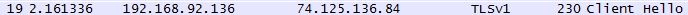
\includegraphics[width=1\linewidth]{ClientHello}}
\caption{Client Hello}
\label{fig:speciation}
\end{figure}

This is the Client Hello packet seen from wireshark. From this we can see the client's ip adress (192.168.92.136) and the server's ip adress (74.125.136.84) and that the recording used TLS instead of SSL.

\vspace{5mm}\hrule\vspace{5mm}
%---------------------

\begin{figure}[H] % TLS verson
\center{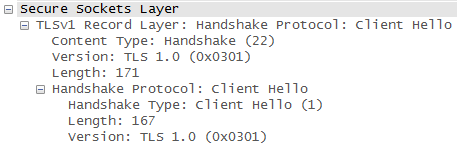
\includegraphics[width=0.8\linewidth]{TLSverson}}
\caption{TLS verson}
\label{fig:speciation}
\end{figure}

Version Number:
Client sends the version number corresponding to the highest version it supports. In this case TLS version 1.0.

\vspace{5mm}\hrule\vspace{5mm}
%---------------------

\begin{figure}[H] % Client Random
\center{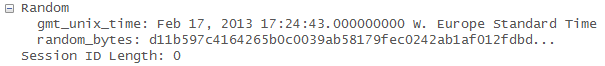
\includegraphics[width=1\linewidth]{ClientRandom}}
\caption{Client Random}
\label{fig:speciation}
\end{figure}

here the cient generates a 32 byte value consisting of a 4-byte number that contains the client’s date and time, plus a 28 byte randomly generated number that ultimately will be used with the server random value to generate a master secret. In this case we can see that the recording was done on feb 17  2013.

\vspace{5mm}\hrule\vspace{5mm}
%---------------------

\begin{figure}[H] % Client Cipher Suits
\center{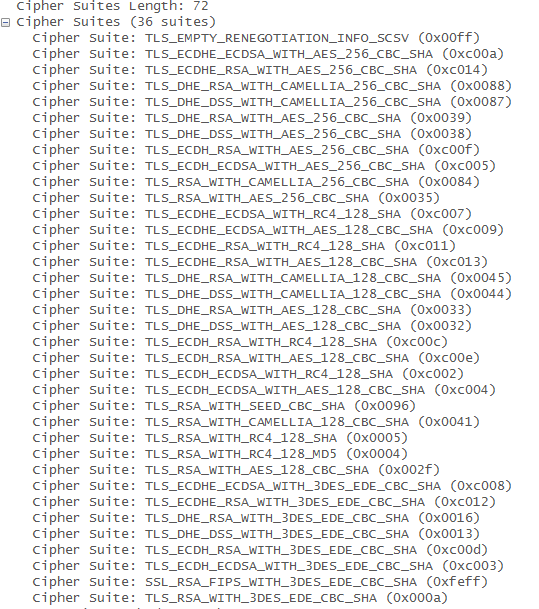
\includegraphics[width=0.8\linewidth]{ClientCipherSuits}}
\caption{Client Cipher Suits}
\label{fig:speciation}
\end{figure}

In this tab we can see that the client sends all the different cipher suits that it is compatible with. Every part of the name describes the different parts the suit is using.
Taking TLS\_RSA\_WITH\_DES\_CBC\_SHA as an example: TLS is the protocol version, RSA is the algorithm that will be used for the key exchange, DES\_CBC is the encryption algorithm (using a 56-bit key in CBC mode), and SHA is the hash function.

\vspace{5mm}\hrule\vspace{5mm}
%---------------------

\begin{figure}[H] % Client Curves
\center{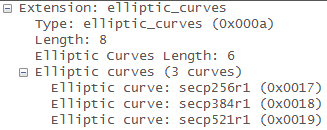
\includegraphics[width=0.5\linewidth]{ClientCurves}}
\caption{Client Curves}
\label{fig:speciation}
\end{figure}

In this recording we can also see that elliptic curves are in use, and here the client sends three different curves that the client supports.

\vspace{5mm}\hrule\vspace{5mm}
%---------------------

\begin{figure}[H] % Client EC Point Format
\center{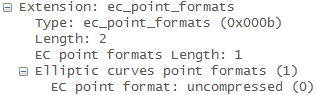
\includegraphics[width=0.6\linewidth]{ClientECPointFormat}}
\caption{Client EC Point Format}
\label{fig:speciation}
\end{figure}

The client EC Point Formats is a list of the point formats a client is able to parse, which the client is required to send with the ClientHello message when it suggests the use of elliptic curves as is the case when using the Elliptic Curve variety of an algorithm such as Diffie-Hellman.

\vspace{5mm}\hrule\vspace{5mm}
%---------------------

%%% Server hello:

\begin{figure}[H] % Server Hello
\center{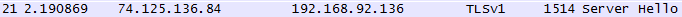
\includegraphics[width=1\linewidth]{ServerHello}}
\caption{Server Hello}
\label{fig:speciation}
\end{figure}

This is the server hello packet seen from wireshark. 

\vspace{5mm}\hrule\vspace{5mm}
%---------------------

\begin{figure}[H] % ServerTLSVerson
\center{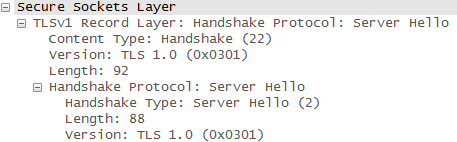
\includegraphics[width=0.8\linewidth]{ServerTLSVerson}}
\caption{Server TLS Verson}
\label{fig:speciation}
\end{figure}

The server sends the highest version number supported by BOTH sides.

\vspace{5mm}\hrule\vspace{5mm}
%---------------------

\begin{figure}[H] % Server Random
\center{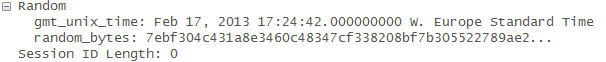
\includegraphics[width=1\linewidth]{ServerRandom}}
\caption{Server Random}
\label{fig:speciation}
\end{figure}

Here the server creates a random number the same way the client did earlier.

\vspace{5mm}\hrule\vspace{5mm}
%---------------------

\begin{figure}[H] % Server Cipher Suite
\center{
\includegraphics[width=0.8\linewidth]{ServerCipherSuite}}
\caption{Server Cipher Suite}
\label{fig:speciation}
\end{figure}

The server will choose the strongest cipher that BOTH the client and server support. In this case its TLS\_ECDHE\_RSA\_WITH\_RC4\_128\_SHA (0xc011).
If no cipher is supported by both the client and server, the session is ended with a “Handshake Failure” alert.

\vspace{5mm}\hrule\vspace{5mm}
%---------------------

\begin{figure}[H] % Server EC Point Formats
\center{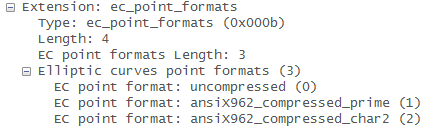
\includegraphics[width=0.8\linewidth]{ServerECPointFormats}}
\caption{Server EC Point Formats}
\label{fig:speciation}
\end{figure}

When the server has received a ClientHello containing a list of elliptic curves and chosen a curve it wishes to use, it's required to use the point format suggested by the client to describe the point on the curve it wishes to use, as well as the curve it wishes to use.

\vspace{5mm}\hrule\vspace{5mm}
%--------------------- %%Certificate:

\begin{figure}[H] % Certificate
\center{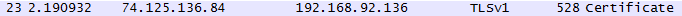
\includegraphics[width=1\linewidth]{Certificate}}
\caption{Certificate}
\label{fig:speciation}
\end{figure}

The server now sends it's Certificate to the client.

\vspace{5mm}\hrule\vspace{5mm}
%---------------------

\begin{figure}[H] % CertificateTLSverson
\center{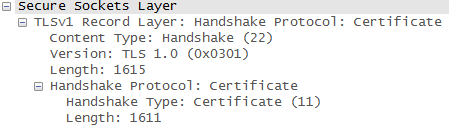
\includegraphics[width=0.8\linewidth]{CertificateTLSverson}}
\caption{Certificate TLS verson}
\label{fig:speciation}
\end{figure}



\vspace{5mm}\hrule\vspace{5mm}
%---------------------

\begin{figure}[H] % CertificateCertificates
\center{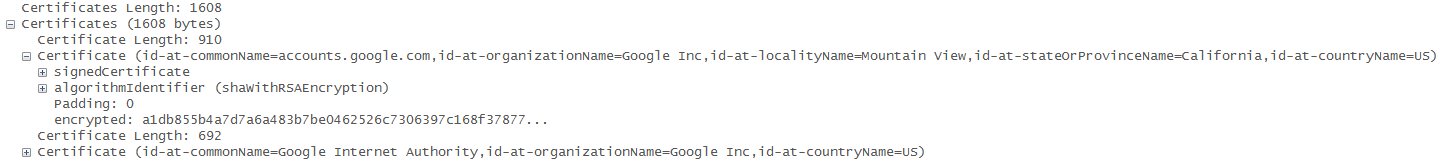
\includegraphics[width=1.2\linewidth]{CertificateCertificates}}
\caption{Certificate Certificates}
\label{fig:speciation}
\end{figure}

In this tab we can see the different certificates the servers send, and all their information (1608bytes). 
On the first line we can se the total lenght of all the certificates in the tab. we can then see the lenght of the first certificate, in the case its 910bytes. After that we see those 910bytes in data form.

\vspace{5mm}\hrule\vspace{5mm}
%---------------------

\begin{figure}[H] % Certificate EC Diffie Hellman Server Params
\center{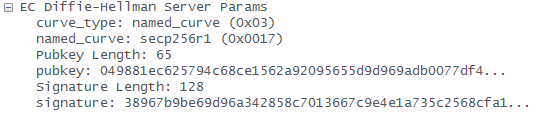
\includegraphics[width=1\linewidth]{CertificateECDiffieHellmanServerParams}}
\caption{Certificate EC Diffie Hellman Server Params}
\label{fig:speciation}
\end{figure}

Here the server sends it's choice out of the curves the client supported. In this case the server chose the secp256r1 curve. 
The server then sends the public key length, followed by the public key.
This message also contains a signature that proves possession of the private key corresponding to client's public key.

\vspace{5mm}\hrule\vspace{5mm}
%---------------------

\begin{figure}[H] % CertificateServerKeyExchange
\center{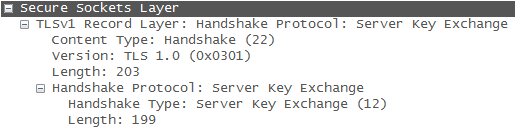
\includegraphics[width=0.8\linewidth]{CertificateServerKeyExchange}}
\caption{Certificate Server Key Exchange}
\label{fig:speciation}
\end{figure}

The server sends it's ephemeral ECDH public key to the client

\vspace{5mm}\hrule\vspace{5mm}
%---------------------

\begin{figure}[H] % Server Hello Done
\center{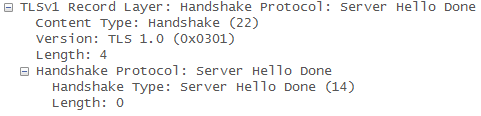
\includegraphics[width=0.8\linewidth]{ServerHelloDone}}
\caption{Server Hello Done}
\label{fig:speciation}
\end{figure}

The server has now told the client that it is done, and are now waiting for a response from the client.
%%% Client key exchange:
\vspace{5mm}\hrule\vspace{5mm}

\begin{figure}[H] % Client Key Exchange
\center{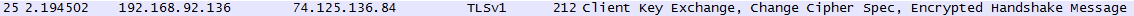
\includegraphics[width=1\linewidth]{ClientKeyExchange}}
\caption{Client Key Exchange}
\label{fig:speciation}
\end{figure}

\vspace{5mm}\hrule\vspace{5mm}
%---------------------

\begin{figure}[H] % Client Key Exchange Verson 
\center{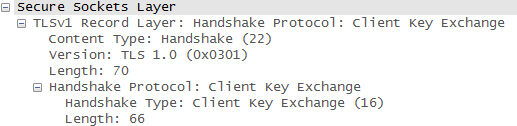
\includegraphics[width=0.8\linewidth]{ClientKeyExchangeVerson}}
\caption{Client Key Exchange Version}
\label{fig:speciation}
\end{figure}

\vspace{5mm}\hrule\vspace{5mm}
%---------------------

\begin{figure}[H] % Client Key Exchange DiffieHellman Client Params
\center{
\includegraphics[width=1\linewidth]{ClientKeyExchangeDiffieHellmanClientParams}}
\caption{Client Key Exchange DiffieHellman Client Params}
\label{fig:speciation}
\end{figure}

The client sends a Client Key Exchange message after computing the premaster secret using both random values.
The premaster secret is encrypted by the public key from the server’s certificate before being transmitted to the server.
Both the client and server will compute the master secret locally and derive the session key from it.

\vspace{5mm}\hrule\vspace{5mm}
%---------------------

\begin{figure}[H] % Client Key Exchange Change Cipher
\center{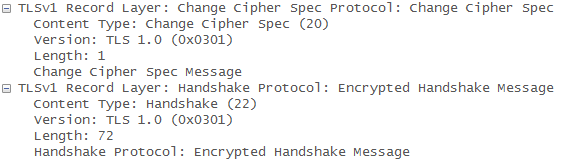
\includegraphics[width=1\linewidth]{ClientKeyExchangeChangeCipher}}
\caption{Client Key Exchange Change Cipher}
\label{fig:speciation}
\end{figure}

This message contains a change cipher spec message, and an encrypted handshake message wich contains a summary of the whole handshake.

\vspace{5mm}\hrule\vspace{5mm}
%---------------------

\begin{figure}[H] % NewSessionTicket
\center{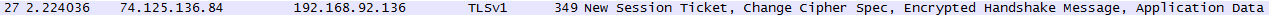
\includegraphics[width=1\linewidth]{NewSessionTicket}}
\caption{New Session Ticket}
\label{fig:speciation}
\end{figure}

The client requests to start a new session after the handshake to transfer data.

\vspace{5mm}\hrule\vspace{5mm}
%---------------------

\begin{figure}[H] % Client Session Ticket
\center{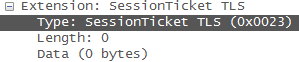
\includegraphics[width=0.6\linewidth]{ClientSessionTicket}}
\caption{Client Session Ticket}
\label{fig:speciation}
\end{figure}

\vspace{5mm}\hrule\vspace{5mm}
%---------------------

\begin{figure}[H] % ApplicationData
\center{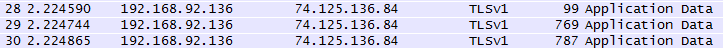
\includegraphics[width=1\linewidth]{ApplicationData}}
\caption{Application Data}
\label{fig:speciation}
\end{figure}

Data packets sent after the TLS handshake is successful.s


%----------------------------------------------------------------------------------------
%	ATTACKS AGAINST SSL (Maybe write a page or two about this subject?)
%----------------------------------------------------------------------------------------
\section {Attacks Against The SSL Protocol}
In the past we have seen a few different attacks targeting the SSL/TLS protocol, including BEAST~\cite{beastattack}, CRIME~\cite{crimeattack} and Lucky 13~\cite{lucky13}.\\
And now, on the 20th International Workshop on Fast Software Encryption and the Blackhat Security conference in Amsterdam this year, two new attacks were presented to the participants.\\
\bigskip
What most of these attacks have in common is that they all are capable of silently decrypting browser cookies used to log in to websites. And obviously this can be a real threat against users of websites which are securing their communication with SSL/TLS.\\
This section will also discuss a method which is using SSL to carry out a DoS attack. This attack vector was discovered and presented back in 2011.

\subsection{BEAST}
In 2011, the two researchers Juliano Rizzo and Thai Duong demonstrated a POC (Proof-of-consept) called Browser Exploit Against SSL/TLS (BEAST). This attack is known as a plaintext-recovery attack.\\
The difference between BEAST and other similar attacks was that this exploit attacked the confidentiality of the SSL/TLS protocol.

''\textit{During the encryption process, the protocol scrambles block after block of data using the previous encrypted block. It has long been theorized that attackers can manipulate the process to make educated guesses about the contents of the plaintext blocks.}''~\cite{theregisterBEAST}

So if an attacker could make a correct guess, he/she would basically break the encryption and thus reveal potientially sensitive data.\\
\bigskip
Before the vulnerability was fixed, BEAST required about 2 seconds to decrypt each byte of a cookie, and since authentication cookies consists of between 1000 and 2000 characters it would take this attack about 10 minutes to work.\\
Needless to say, this attack was a gigantic threat against websites that used an early version of TLS, and it obviously came as a shock to people who were working in the security field at that time.

\subsection{Cipher Suite Rollback}
When a client starts the SSL Handshake with the server, the client sends a list over all the cipher suits it supports. The server then chooses the strongest cipher suite both parties support.\\
With a Cipher Suite Rollback Attack~\cite{sslrollbackattack}, an attacker can intercept the handshake, and send a list over weak and old cipher suit on behalf of the client, and thus ''forcing'' the client and server to use a weak encryption algorithm during the communication.\\
The attacker can then take advantage of this, and in the worst case scenario obtain sensitive data and/or credentials.

\subsection{SSL DDoS Attack}
In traditional DoS/DDoS attacks the attacker will send massive amounts of data to the server and essentially take down the server and prevent other users from accessing the content. But in 2011 a group of researchers found a more clever way to perform a DoS/DDoS attack.\\
When the client establish a connection to a server using a SSL connection iit requires about 15 times more processing power on the server than on the client. So by opening thousand of SSL connections the server's processor will eventually get overloaded, thus resulting in a successfull attack.\\
\bigskip
An ethical hacker that runs Darknet came up with a few different tips towards completing a successfull SSL DoS attack~\cite{sslddosattack}:
\begin{itemize}
\item The average server can do 300 handshakes per second. This would require 10-25\% of your laptops CPU
\item Use multiple hosts (SSL-DOS) if an SSL Accelaretor is used.
\item Don't rely on just port 443 (HTTPS). Test other ports as well; (SMTP, POP3S).
\end{itemize}

%----------------------------------------------------------------------------------------
%       GRAPHICAL REPRESENTATION
%----------------------------------------------------------------------------------------
\section{Graphical Representation}

\begin{figure}[H] % SSL Handshake
\center{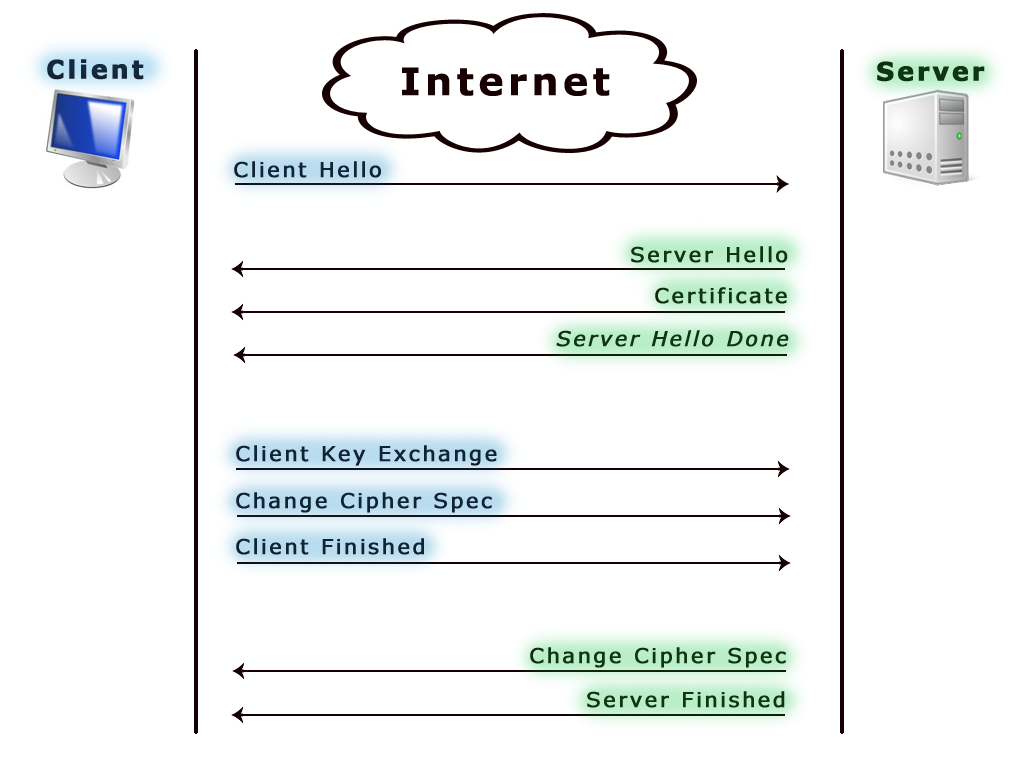
\includegraphics[width=1\linewidth]{SSL_handshake_image}}
\caption{SSL Handshake}
\label{fig:speciation}
\end{figure}

The graphic above shows how the SSL handshake is performed.

\begin{figure}[H] % SSL connection process
\center{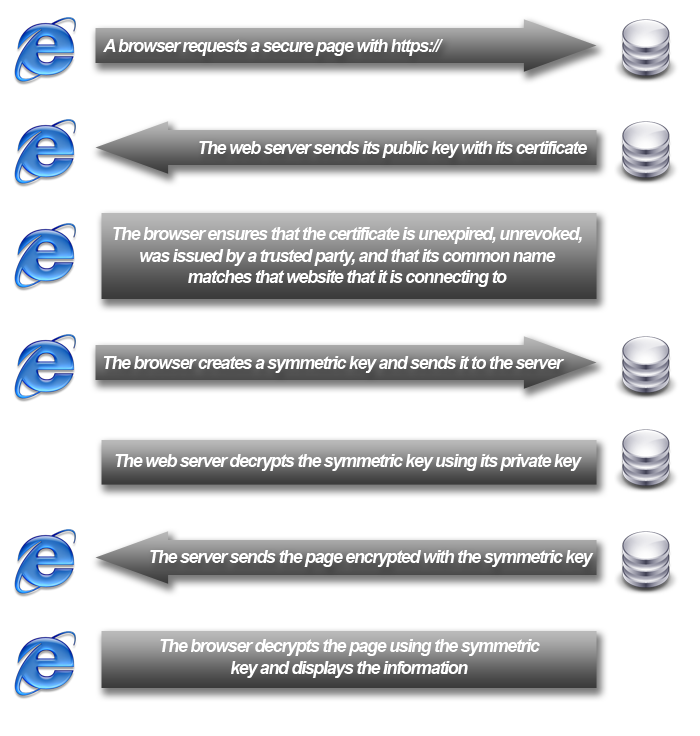
\includegraphics[width=1\linewidth]{what-is-ssl-connection-process}}
\caption{SSL connection process\cite{SSL_connection_process}}
\label{fig:speciation}
\end{figure}

The graphic above discribes the SSL connection process, and how the browser communicates with the server.

\begin{figure}[H] % Asymmetric encryption
\center{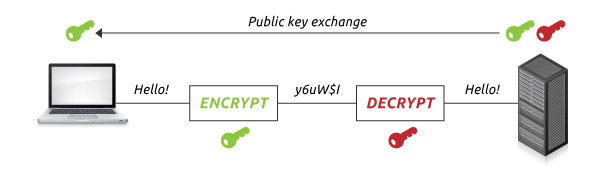
\includegraphics[width=0.8\linewidth]{Asymmetric_encryption}}
\caption{Asymmetric encryption\cite{Asymmetric_encryption}}
\label{fig:speciation}
\end{figure}

Graphical description of Asymmetric encryption in a very basic way.

\vspace{5mm}\hrule\vspace{5mm}

\begin{figure}[H] % symmetric encryption
\center{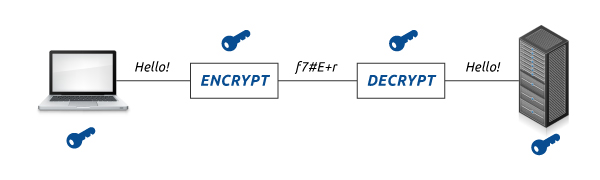
\includegraphics[width=0.8\linewidth]{symmetric_encryption}}
\caption{Symmetric encryption\cite{Symmetric_encryption}}
\label{fig:speciation}
\end{figure}

Graphical description of Symmetric encryption in a very basic way.

\begin{figure}[H] % PKI overview
\center{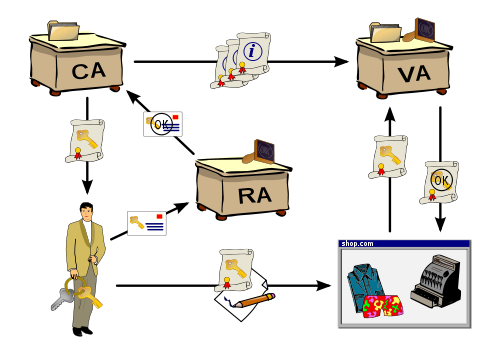
\includegraphics[width=0.8\linewidth]{pki-overview}}
\caption{PKI overview\cite{pki_overview}}
\label{fig:speciation}
\end{figure}

\vspace{5mm}\hrule\vspace{5mm}

This graphic shows an overview of a Public-key innfrastructure.

\begin{figure}[H] % Green bar overview
\center{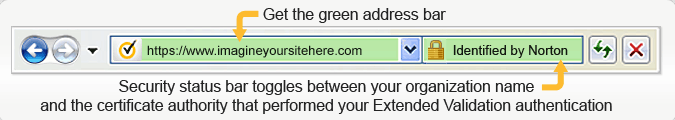
\includegraphics[width=1\linewidth]{green_bar}}
\caption{Green bar overview\cite{green_bar}}
\label{fig:speciation}
\end{figure}

This figure shows how some SSL certificates (often the highest trust-level) affects the users browser client.

%----------------------------------------------------------------------------------------
%	BIBLIOGRAPHY (References)
%----------------------------------------------------------------------------------------
\bibliographystyle{unsrt}
\bibliography{Sources}
%\begin{thebibliography}{99} % Bibliography - this is intentionally simple in this template

%\bibitem[Figueredo and Wolf, 2009]{Figueredo:2009dg}
%Figueredo, A.~J. and Wolf, P. S.~A. (2009).
%\newblock Assortative pairing and life history strategy - a cross-cultural
%  study.
%\newblock {\em Human Nature}, 20:317--330.
 
%\end{thebibliography}

%----------------------------------------------------------------------------------------------------------------------------------------------------
\end{document}